%----------------------------------------------------------------------------------------
%    PACKAGES AND THEMES
%----------------------------------------------------------------------------------------

\documentclass[aspectratio=169,xcolor=dvipsnames]{beamer}
\usetheme{SimpleDarkBlue}
\usepackage{multicol}
\usepackage{hyperref}
\usepackage{graphicx}
\usepackage{booktabs}
\usepackage{tikz}
\usetikzlibrary{positioning, arrows}
\usepackage{ragged2e}

%----------------------------------------------------------------------------------------
%    HYPERREF SETUP (NO WARNINGS)
%----------------------------------------------------------------------------------------

\hypersetup{
    pdftitle={Interpretable Lightweight Transformer via Unrolling of Learned Graph Smoothness Priors},
    pdfauthor={Kenneth Browder and Fabien Lagnieu},
    pdfsubject={Final Report - Machine Learning with Graphs - IPP 2025},
    pdfkeywords={Graph Signal Processing, Transformers, GSP, Unrolling, Interpretability}
}

%----------------------------------------------------------------------------------------
%    TITLE PAGE
%----------------------------------------------------------------------------------------

\title{Interpretable Lightweight Transformer via \\ Unrolling of Learned Graph Smoothness Priors}
\subtitle{Tam Thuc Do, Parham Eftekhar, Seyed Alireza Hosseini, Gene Cheung, Philip Chou\\ ___ \\ \textbf{Final Report Presentation} \\ Machine Learning with Graphs - IPP 2025}

\author{Kenneth Browder - Fabien Lagnieu}
\institute{Institut Polytechnique de Paris}
\date{April 1, 2025}

%----------------------------------------------------------------------------------------
%    PRESENTATION SLIDES
%----------------------------------------------------------------------------------------

\begin{document}

%------------------------------------------------
% Title Page
%------------------------------------------------

\begin{frame}
    \titlepage
    \begin{center}
        
\includegraphics[width=0.7\linewidth]{IPP-Horizontal.png}
    \end{center}
\end{frame}

%------------------------------------------------
% Agenda
%------------------------------------------------

\begin{frame}{Agenda}
    \tableofcontents
\end{frame}

%------------------------------------------------
\section{Context \& Motivation}

\begin{frame}{1. Context \& Motivation}

    \begin{columns}[c] % Alignement centré
        %---------------------------
        \column{0.6\textwidth} % Partie texte à gauche
        \begin{itemize}
            \item \textbf{Transformers} are state-of-the-art in NLP \& CV but suffer from:
            \begin{itemize}
                \item High computational cost
                \item Lack of interpretability
            \end{itemize}
            \vspace{0.5cm}
            \item The paper proposes an \textbf{interpretable and lightweight} model:
            \begin{itemize}
                \item Combining \textbf{Graph Signal Processing (GSP)}
                \item And \textbf{unrolled optimization}
            \end{itemize}
        \end{itemize}

        %---------------------------
        \column{0.4\textwidth} % Partie image à droite
        \begin{figure}
            \centering
            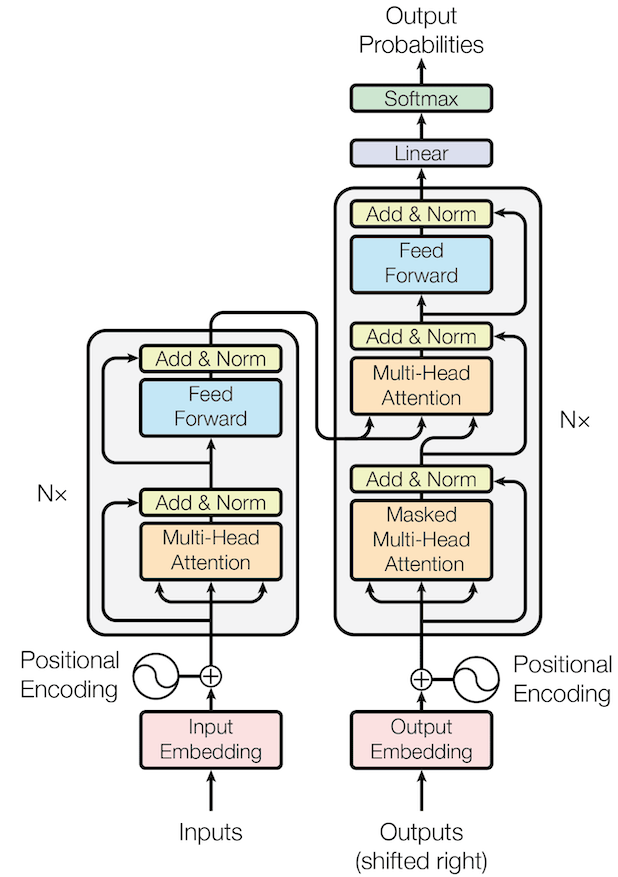
\includegraphics[width=0.8\linewidth]{transformers.png}
            \tiny Transformer architecture (\cite{vaswani2017attention}).
        \end{figure}

    \end{columns}

\end{frame}

%------------------------------------------------
\section{State of the Art}

\begin{frame}{2. State of the Art}
    \begin{itemize}
        \item \textbf{Graph Neural Networks (GNNs)}  
        \\Learn node and graph-level representations through message passing.
        \begin{itemize}
            \item Powerful but complex and hard to interpret.
            \item Struggle with scalability and over-smoothing in deep architectures.
        \end{itemize}

        \vspace{0.4cm}
        \item \textbf{Graph Signal Processing (GSP)}  
        \\Provides well-defined priors for graph data.
        \begin{itemize}
            \item \textbf{Graph Laplacian Regularizer (GLR)}: enforces smoothness across the graph. \cite{ortega2018graph}
            \item \textbf{Graph Total Variation (GTV)}: preserves edges and discontinuities. \cite{cheung2018graph}
        \end{itemize}

        \vspace{0.4cm}
        \item \textbf{Optimization Unrolling (brief)}  
        \\Converts iterative optimization algorithms into neural network layers.
        \begin{itemize}
            \item Improves interpretability and model efficiency.
        \end{itemize}
    \end{itemize}
\end{frame}
%------------------------------------------------
\section{Main Contributions}

\begin{frame}{3. Main Contributions}
    \begin{itemize}
        \item \textbf{Transformer-like architecture via optimization unrolling}
        \begin{itemize}
            \item Each layer corresponds to an iteration of an optimization algorithm.
            \item Brings interpretability to layer operations and reduces computational cost.
        \end{itemize}

        \vspace{0.3cm}

        \item \textbf{Mahalanobis distance-based graph learning}
        \begin{itemize}
            \item Learns a similarity graph by adapting the Mahalanobis distance. \cite{hu2020feature}
            \item Ensures symmetric adjacency and interpretable edge weights.
        \end{itemize}

        \vspace{0.3cm}

        \item \textbf{Lightweight, interpretable, and efficient for graph signal interpolation}
        \begin{itemize}
            \item Achieves state-of-the-art performance with significantly fewer parameters.
            \item Demonstrates robustness and generalization across tasks.
        \end{itemize}
    \end{itemize}
\end{frame}
%------------------------------------------------
%------------------------------------------------
\section{Methodology}

\begin{frame}{4. Methodology Overview}
    \begin{itemize}
        \item \textbf{Alternating graph learning and signal interpolation}
        \begin{itemize}
            \item At each layer, the similarity graph and node features are jointly refined.
        \end{itemize}

        \vspace{0.2cm}

        \item \textbf{Unrolled optimization replacing attention mechanisms}
        \begin{itemize}
            \item Conjugate Gradient (GLR) and ADMM (GTV) unfold as layers.
            \item Each iteration is explicitly controlled and interpretable.
        \end{itemize}
    \end{itemize}

    \vspace{0.2cm}

    \begin{figure}
        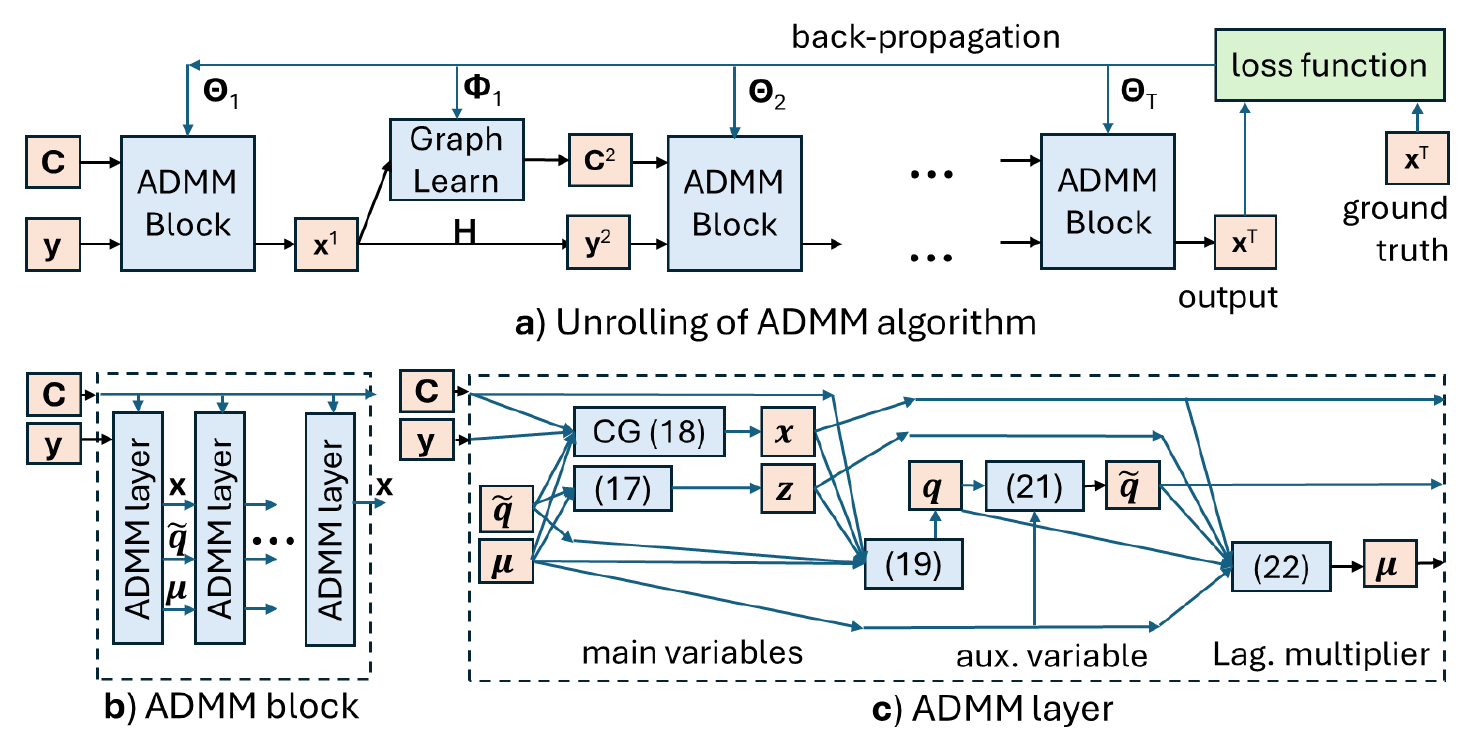
\includegraphics[width=0.5\linewidth]{GTV-based_algorithm.png}
        \\\tiny GTV-based unrolled algorithm \cite{do2024interpretable}
    \end{figure}
\end{frame}

%------------------------------------------------
\begin{frame}{4.1 Graph Learning via Mahalanobis Distance}

\begin{columns}[c]

% LEFT COLUMN
\begin{column}{0.6\textwidth}

\begin{itemize}
    \item Learn a similarity graph $\rightarrow$ pairwise distances.
    
    \item Mahalanobis distance: \cite{hu2020feature}
    \[
        d(i, j) = (\mathbf{f}_i - \mathbf{f}_j)^\top M (\mathbf{f}_i - \mathbf{f}_j)
    \]
    
    \item $M$ is a learnable, positive semi-definite matrix.
    
    \item Output edge weights:
    \[
        w_{ij} = \exp(-d(i, j))
    \]
    
    \item Local Softmax normalization:
    \[
        w_{ij} = \frac{\exp(-d(i, j))}{\sum_{j' \in \mathcal{N}(i)} \exp(-d(i, j'))}
    \]
\end{itemize}

\end{column}

% RIGHT COLUMN
\begin{column}{0.4\textwidth}

\begin{center}
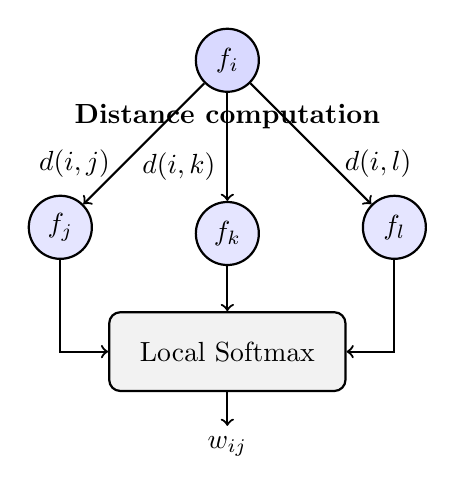
\begin{tikzpicture}[node distance=1.2cm, auto, thick]

% Central node f_i on top
\node[draw, circle, minimum size=0.8cm, fill=blue!15] (i) {$f_i$};

% Neighbor nodes below
\node[draw, circle, minimum size=0.8cm, fill=blue!10, below left of=i, node distance=3cm] (j) {$f_j$};
\node[draw, circle, minimum size=0.8cm, fill=blue!10, below of=i, node distance=2.2cm] (k) {$f_k$};
\node[draw, circle, minimum size=0.8cm, fill=blue!10, below right of=i, node distance=3cm] (l) {$f_l$};

% Arrows from i to neighbors with distances
\node[below=0.01cm of i, draw=none] (distlabel) {\textbf{Distance computation}};
\draw[->] (i) -- node[left, yshift=-0.25cm, xshift=-0.3cm] {$d(i,j)$} (j);
\draw[->] (i) -- node[right, yshift=-0.25cm, xshift=0.3cm] {$d(i,l)$} (l);
\draw[->] (i) -- node[left, yshift=-0.25cm, xshift=-0.02cm] {$d(i,k)$} (k);

% Softmax box under neighbors
\node[draw, rounded corners, minimum width=3cm, minimum height=1cm, below of=k, node distance=1.5cm, fill=gray!10] (softmax) {Local Softmax};

% Arrows from neighbors to softmax
\draw[->] (j) |- (softmax);
\draw[->] (k) -- (softmax);
\draw[->] (l) |- (softmax);

% Output
\node[below of=softmax, node distance=1.2cm] (output) {$w_{ij}$};
\draw[->] (softmax) -- (output);

\end{tikzpicture}
    \begin{figure}
        \tiny Learned edge weights $w_{ij}$ based on Mahalanobis distance and local softmax normalization.
    \end{figure}
\end{center}

\end{column}

\end{columns}

\end{frame}


%------------------------------------------------
\begin{frame}{4.2 Signal Interpolation via Unrolled Optimization}

\begin{columns}[c]

% Left column: explanation
\begin{column}{0.51\textwidth}

\begin{itemize}
    \item After graph learning, node signals are interpolated: \textbf{two methods}
    \begin{itemize}
        \item \textbf{GLR}: Conjugate Gradient (CG) \cite{shewchuk1994introduction}
        \item \textbf{GTV}: Alternating Direction Method of Multipliers (ADMM) \cite{wang2017new}
    \end{itemize}
    \vspace{0.05cm}
    \item \textbf{Unrolled optimization}:  
    Each layer corresponds to an iteration, enabling interpretability and convergence control.
    \vspace{0.05cm}
    \item \textbf{Output}: High-quality, edge-preserving interpolation on graph signals.
\end{itemize}

\end{column}

% Right column: diagram
\begin{column}{0.47\textwidth}

\begin{center}
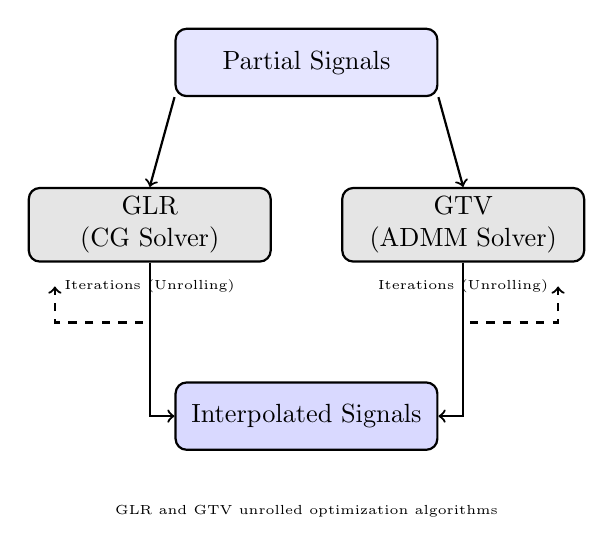
\begin{tikzpicture}[node distance=1.2cm, thick, scale=0.95, every node/.style={transform shape}]

% Input signals block
\node[draw, rounded corners, fill=blue!10, minimum width=3.5cm, minimum height=0.9cm] (input) {Partial Signals};

% GLR and GTV Blocks (closer)
\node[draw, rounded corners, fill=gray!20, minimum width=3cm, minimum height=0.9cm, below left=1.2cm and -1.3cm of input, text width=3cm, align=center] (glr) {GLR \\ (CG Solver)};
\node[draw, rounded corners, fill=gray!20, minimum width=3cm, minimum height=0.9cm, below right=1.2cm and -1.3cm of input, text width=3cm, align=center] (gtv) {GTV \\ (ADMM Solver)};

% Arrows from input to solvers
\draw[->, thick] (input.south west) -- (glr.north);
\draw[->, thick] (input.south east) -- (gtv.north);

% Output signals block
\node[draw, rounded corners, fill=blue!15, minimum width=3.5cm, minimum height=0.9cm, below=3.8cm of input] (output) {Interpolated Signals};

% Arrows from solvers to output
\draw[->, thick] (glr.south) |- (output.west);
\draw[->, thick] (gtv.south) |- (output.east);

% Iterative arrows to symbolize unrolling
\node[below=0.1cm of glr] (glrtext) {\tiny Iterations (Unrolling)};
\draw[dashed, ->] (glr.south) -- ++(0,-0.8) -| (glrtext.west);

\node[below=0.1cm of gtv] (gtvtext) {\tiny Iterations (Unrolling)};
\draw[dashed, ->] (gtv.south) -- ++(0,-0.8) -| (gtvtext.east);

% Caption
\node[below=0.6cm of output] {\tiny GLR and GTV unrolled optimization algorithms};

\end{tikzpicture}
\end{center}

\end{column}

\end{columns}

\end{frame}


%------------------------------------------------
%------------------------------------------------
\section{Paper Experimentation}

\begin{frame}{5.1 Experimental Setup}

\begin{itemize}
    \item \textbf{Training Dataset: DIV2K}
    \begin{itemize}
        \item 800 HR images for training, 100 for validation
        \item Extracted $64 \times 64$ patches, using only 1\% - 4\% for training
    \end{itemize}
    
    \item \textbf{Test Datasets}
    \begin{itemize}
        \item McM \cite{zhang2011color}
        \item Kodak  \cite{kodak1993} 
        \item Urban100 \cite{huang2015single}.
    \end{itemize}
    
    \item \textbf{Tasks}
    \begin{itemize}
        \item \textbf{Demosaicking}: reconstruct RGB images from Bayer pattern
        \item \textbf{Image Interpolation}: reconstruct HR images from LR inputs
    \end{itemize}
    
    \item \textbf{Evaluation Metrics}
    \begin{itemize}
        \item Peak Signal-to-Noise Ratio (PSNR)
        \item Structural Similarity Index Measure (SSIM) \cite{wang2004image}
    \end{itemize}
    
    % Optional line about hardware
    % \item \textbf{Implementation:} PyTorch, trained on NVIDIA RTX 2080 Ti
\end{itemize}

\end{frame}

%------------------------------------------------
%------------------------------------------------

\begin{frame}{5.2 Experimental Results}

\begin{columns}[c]

% Left Column - Demosaicking Results
\begin{column}{0.48\textwidth}
    \textbf{Demosaicking} \\[0.2cm]
    
    \begin{center}
        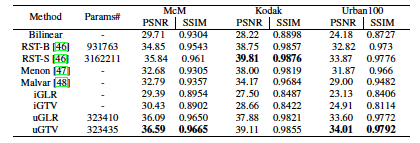
\includegraphics[width=\linewidth]{Demosaicking_results.png}
    \end{center}

    \vspace{0.2cm}
    \begin{itemize}
        \item \textbf{uGTV} achieves top PSNR and SSIM on Urban100 \& McM.
        \item Nearly matches RST-S on Kodak with far fewer parameters.
    \end{itemize}
\end{column}

% Right Column - Image Interpolation Results
\begin{column}{0.48\textwidth}
    \textbf{Image Interpolation} \\[0.2cm]

    \begin{center}
        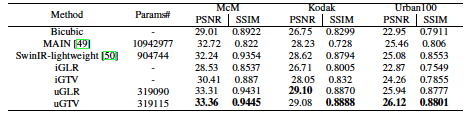
\includegraphics[width=\linewidth]{Interpolation_results.png}
    \end{center}

    \vspace{0.2cm}
    \begin{itemize}
        \item \textbf{uGTV} consistently outperforms SOTA models across datasets.
        \item Maintains efficiency with only 300k parameters versus multi-million parameter baselines.
    \end{itemize}
\end{column}

\end{columns}

\end{frame}

%------------------------------------------------
\begin{frame}{6.1 Experiment 1: Reproducing the Paper Setup}
\footnotesize % encore plus compact

\begin{columns}[T] % alignement en haut

% Left Column - All content
\begin{column}{0.55\textwidth}

\textbf{Objective}
\vspace{-0.1cm}
\begin{itemize}
    \setlength\itemsep{2pt}
    \item Validate uGLR on Div2K dataset
    \item Upscaling: from 32×32 to 64×64
    \item One pixel out of four is retained
\end{itemize}

\textbf{Methodology}
\vspace{-0.1cm}
\begin{itemize}
    \setlength\itemsep{2pt}
    \item No official code found  
    $\rightarrow$ Full reimplementation in PyTorch
    \item CG and ADMM coded from scratch
    \item Sparse ops via PyTorch only
    \item Hardware: A100 (40 GB VRAM)
\end{itemize}

\textbf{Model Parameters}
\vspace{-0.1cm}
\begin{itemize}
    \setlength\itemsep{2pt}
    \item $64 \times 64$ images $\Rightarrow$ 4096 nodes
    \item $5 \times 5$ neighborhood ($\sim$24 edges/node)
    \item ADMM block: 5 layers × 10 CG steps
    \item CNN: 4 layers, 48 features $\rightarrow$ 4×12 heads
\end{itemize}

\end{column}

% Right Column - Image
\begin{column}{0.50\textwidth}

\textbf{Discussion}
\vspace{-0.1cm}
\begin{itemize}
    \setlength\itemsep{2pt}
    \item $\sim10^5$ edges $\Rightarrow$ GPU overflow
    \item Sparse ops needed but PyTorch support limited
    \item Batched design complicated sparse integration
    \item Reproduction failed due to memory limits
\end{itemize}

\begin{center}
\vspace{0.2cm}
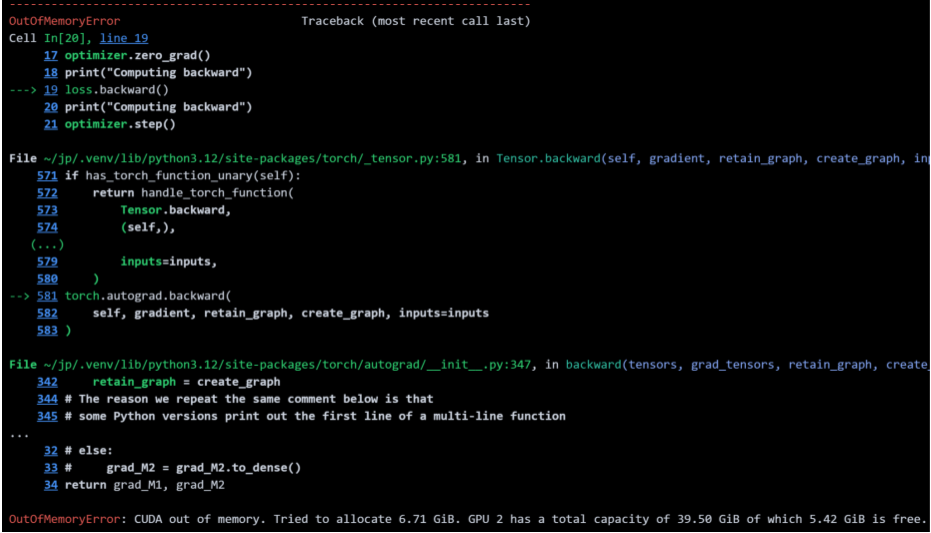
\includegraphics[width=0.95\linewidth]{OutofMemory.png}
\vspace{-0.2cm}
\tiny CUDA Out-of-Memory on A100 (loss.backward step)
\end{center}
\end{column}

\end{columns}
\end{frame}


%---------------------------------------------------------------------------------------
\begin{frame}{6.2 Experiment 2: Scaled-Down Model on 32×32 Images}


\begin{columns}[T]

% Left Column - Text
\begin{column}{0.50\textwidth}

\textbf{Objective}
\vspace{-0.1cm}
\begin{itemize}
    \setlength\itemsep{2pt}
    \item Train a reduced uGLR model for image upscaling
    \item Input: 32×32 image, Output: 64×64
\end{itemize}

\textbf{Methodology}
\vspace{-0.1cm}
\begin{itemize}
    \setlength\itemsep{2pt}
    \item Same PyTorch implementation as before
    \item Lowered model complexity for memory feasibility
    \item Fewer features, fewer neighbors per node
\end{itemize}

\textbf{Remarks}
\vspace{-0.1cm}
\begin{itemize}
    \setlength\itemsep{2pt}
    \item Successfully trained on constrained hardware
    \item Visual inspection confirms signal reconstruction
    \item Results not directly comparable to paper metrics
\end{itemize}

\end{column}

% Right Column - Diagram
\begin{column}{0.55\textwidth}
\begin{center}

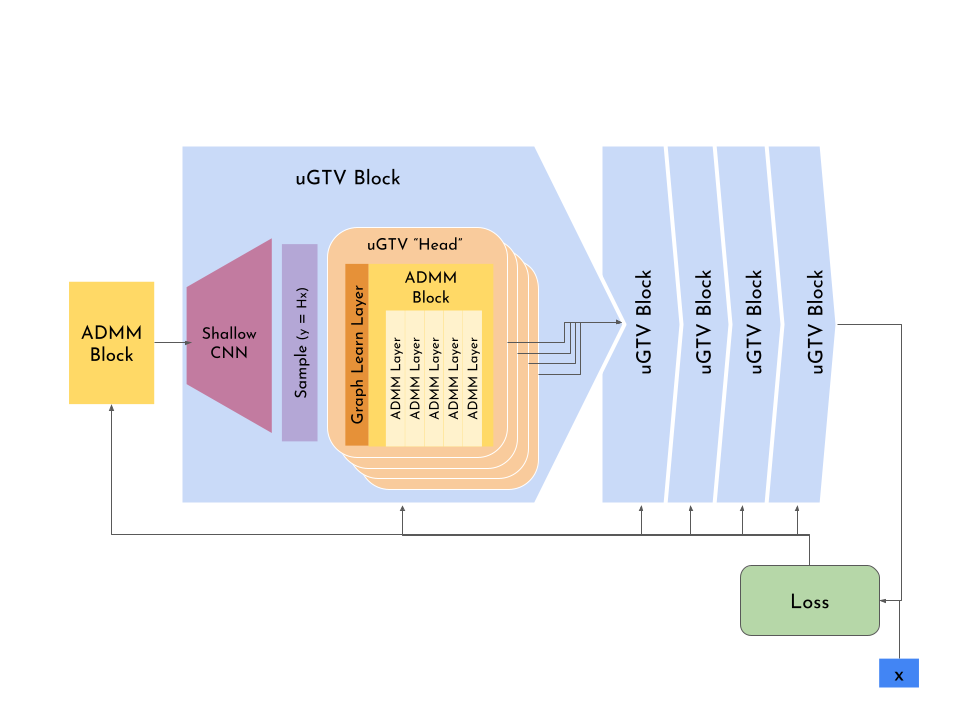
\includegraphics[width=1\linewidth]{Method Diagram .png}


\tiny \textit{Reduced uGLR architecture used in additional experiment}
\end{center}
\end{column}

\end{columns}
\end{frame}

%------------------------------------------------
\section{Critical Analysis}

\begin{frame}{7. Critical Analysis}

    \begin{exampleblock}{Strengths}
        \begin{itemize}
            \item \textbf{Interpretability}: Each layer has a clear mathematical meaning, making the model transparent and easier to analyze.
            
            \item \textbf{Efficiency}: The architecture drastically reduces the number of parameters.
            
            \item \textbf{Strong Results}: Achieves state-of-the-art performance on demosaicking and image interpolation tasks, with robust generalization across datasets.
        \end{itemize}
    \end{exampleblock}

    \begin{alertblock}{Limitations \& Future Work}
        \begin{itemize}
            \item \textbf{Scalability}: The model’s performance and efficiency on very large graphs (e.g., social networks or biological networks) remain unexplored.
            
            \item \textbf{Task Diversity}: The method was only evaluated on image-based interpolation; its applicability to other tasks (e.g., node classification, link prediction) is uncertain.
            
        \end{itemize}
    \end{alertblock}

\end{frame}
%------------------------------------------------
\section{Conclusion \& Questions}

\begin{frame}{8. Conclusion \& Questions}

    \begin{block}{Key Takeaways}
        \begin{itemize}
            \item Introduced an interpretable, lightweight transformer-like model for graph signal interpolation.
            \item Combines Graph Signal Processing with unrolled optimization (GLR / GTV priors).
            \item Achieves state-of-the-art results with significantly fewer parameters.
            \item Demonstrates robustness and efficiency on image-based tasks.
        \end{itemize}
    \end{block}

    \centering
    \Huge{\textbf{Thank You!}} \\
    \vspace{0.2cm}
    \normalsize Questions?
    \vspace{0.2cm}
    \begin{center}
        
\includegraphics[width=0.7\linewidth]{IPP-Horizontal.png}
    \end{center}
\end{frame}

%---------------------------------------------------------------------------------------
\begin{frame}{References}
    \tiny % ou \scriptsize si tu préfères
\begin{justify}
\begin{flushleft}
    \begin{multicols}{2}
        \bibliographystyle{apalike}
        \bibliography{references}
    \end{multicols}
\end{flushleft}
\end{justify}
\end{frame}

%---------------------------------------------------------------------------------------
\begin{frame}{Key Concepts: Graph Signal Processing (GSP)}

\begin{columns}[c]

% Left column: Definitions
\begin{column}{0.60\textwidth}

\begin{itemize}
    \item \textbf{GSP} extends traditional signal processing to irregular domains represented as graphs.
    
    \item A graph $\mathcal{G} = (\mathcal{V}, \mathcal{E})$ consists of nodes $\mathcal{V}$ and edges $\mathcal{E}$, typically described by an adjacency matrix $A$ or Laplacian $L$.
    
    \vspace{0.3cm}
    
    \item \textbf{Graph signals}: data defined on graph nodes (e.g., image pixels, sensors in a network).

    \vspace{0.3cm}
    
    \item \textbf{Key operations}:
    \begin{itemize}
        \item \textbf{Graph Fourier Transform (GFT)}: analyzes signals in the graph spectral domain.
        \item \textbf{Graph Filtering}: smooths or enhances graph signals by manipulating graph frequencies.
        \item \textbf{Graph Laplacian}: central operator for defining smoothness and spectral properties.
    \end{itemize}

    \vspace{0.3cm}

\end{itemize}

\end{column}

% Right column: Illustration
\begin{column}{0.45\textwidth}

\begin{itemize}
    \item \textbf{In this paper}:
    \begin{itemize}
        \item GSP provides priors for signal smoothness over learned graphs.
        \item It ensures edge-aware filtering, improving interpolation tasks.
    \end{itemize}
    
\end{itemize}
\vspace{0.5cm}
\begin{center}
    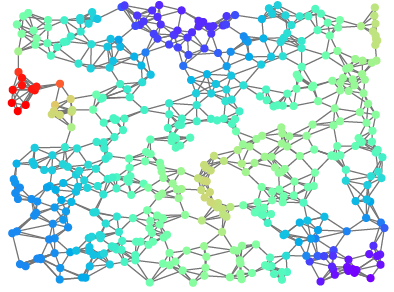
\includegraphics[width=0.65\linewidth]{GSP.png}
    
    \vspace{0.1cm}
    \tiny Graph signals on nodes, smoothness across edges.
\end{center}

\end{column}

\end{columns}

\end{frame}

%---------------------------------------------------------------------------------------
\begin{frame}{Key Concepts: Graph Laplacian Regularizer (GLR)}

\begin{itemize}
    \item \textbf{Objective:} Encourage smoothness of signals across the graph by penalizing differences between neighboring nodes.
    

    \item \textbf{Smoothness assumption:} Connected nodes should have similar signal values.
    

    \item \textbf{GLR formula:}
    \vspace{-0.3cm}
    \[
        \text{GLR}(\mathbf{x}) = \mathbf{x}^\top L \mathbf{x} = \sum_{i,j} w_{ij} (x_i - x_j)^2
    \]
    \vspace{-0.5cm}
    \begin{itemize}
        \item $L$ is the \textbf{graph Laplacian}: $L = D - W$
        \item $W$ is the adjacency matrix (weights $w_{ij}$)
        \item $D$ is the degree matrix
    \end{itemize}
    
    \item \textbf{In this paper:} GLR is unrolled via Conjugate Gradient (CG) optimization to refine signals layer by layer.

\end{itemize}

\begin{center}
    \includegraphics[width=0.55\linewidth]{smoothness.png}
    \vspace{0.2cm}
    \\\tiny \textit{Illustration of graph signals with varying levels of smoothness.}
\end{center}


\end{frame}
%---------------------------------------------------------------------------------------
\begin{frame}{Key Concepts: Graph Total Variation (GTV)}

\begin{columns}[c]

% Left column: Definitions & Explanations
\begin{column}{0.58\textwidth}

\begin{itemize}
    \item \textbf{Objective:} Promote piecewise-smooth signals while preserving sharp edges or discontinuities on the graph.
    
    \item \textbf{Key Idea:} Unlike GLR, GTV tolerates sharp signal changes.
    
    \item \textbf{Mathematical expression:}
    \[
        \text{GTV}(\mathbf{x}) = \sum_{i,j} w_{ij} |x_i - x_j|
    \]
    \vspace{-0.5cm}
    \item \textbf{In this paper:}
    \begin{itemize}
        \item Solved via ADMM, unrolled as layers.
        \item Enables edge-preserving interpolation.
    \end{itemize}
    \item \textbf{Use cases:}  
    Useful in tasks requiring edge preservation, such as image denoising, segmentation, and interpolation.

\end{itemize}

\end{column}

% Right column: Illustration
\begin{column}{0.4\textwidth}

\begin{center}
    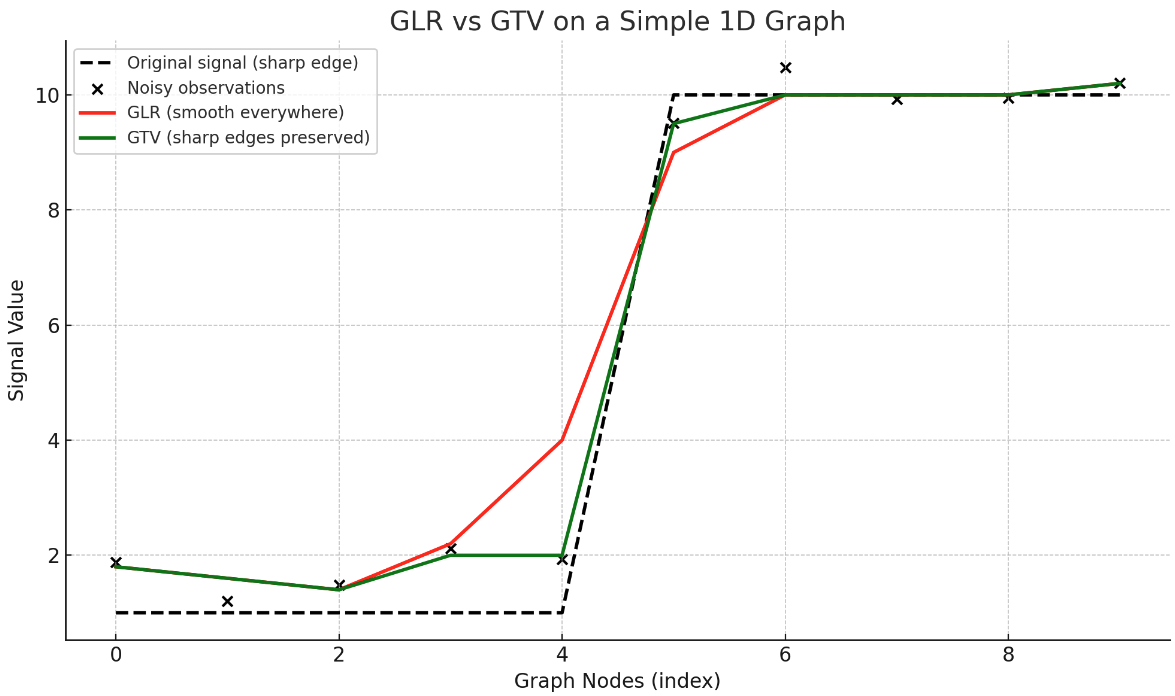
\includegraphics[width=0.95\linewidth]{GLRvsGTV.png}
    \vspace{0.3cm}

    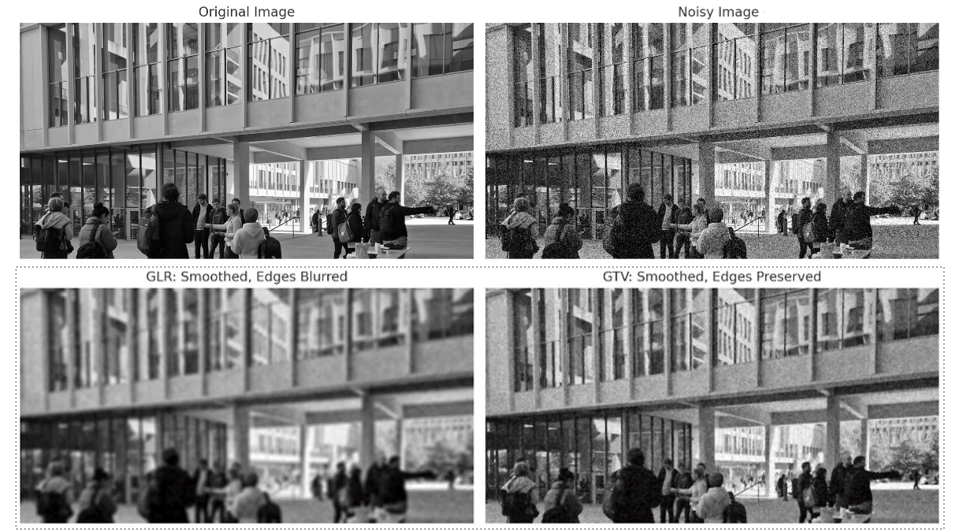
\includegraphics[width=0.95\linewidth]{GLR_vs_GTV_Image.png}
    \vspace{0.1cm}
    \tiny \textit{Difference GLR/GTV: GTV preserves edges.}
\end{center}

\end{column}

\end{columns}

\end{frame}


%---------------------------------------------------------------------------------------
\begin{frame}{Key Concepts: Mahalanobis Distance in Graph Learning}

\begin{columns}[c]

% LEFT COLUMN
\begin{column}{0.45\textwidth}

\begin{itemize}
    \item \textbf{Purpose:} Measure similarity between nodes by considering feature correlations.
    
    
    \item \textbf{Mahalanobis Distance (MD):}
    \[
        MD(\mathbf{x}, \mu) = \sqrt{(\mathbf{x} - \mu)^\top S^{-1} (\mathbf{x} - \mu)}
    \]
    \vspace{-0.4cm}
    \begin{itemize}
        \item $\mu$ is the mean of the distribution.
        \item $S$ is the covariance matrix (captures feature correlations).
    \end{itemize}
    
    
    \item \textbf{Why MD instead of Euclidean?}
    \begin{itemize}
        \item MD accounts for feature scaling and correlations.
        \item More appropriate for high-dimensional, correlated data.
    \end{itemize}

\end{itemize}

\end{column}

% RIGHT COLUMN
\begin{column}{0.55\textwidth}


\textbf{In this paper:}
\begin{itemize}
    \item Mahalanobis distance is \textbf{learned} via a matrix $M$, which is positive semi-definite.
    
    
    \item It defines adaptive edge weights in the similarity graph as  
    $w_{ij} = \exp(-d(i,j))$,  
    where $d(i,j) = (\mathbf{f}_i - \mathbf{f}_j)^\top M (\mathbf{f}_i - \mathbf{f}_j)$.
    
    
    \item This ensures the learned graph structure reflects the underlying data geometry.
\end{itemize}


\begin{center}
    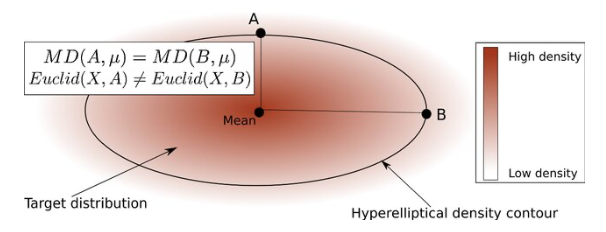
\includegraphics[width=0.7\linewidth]{Mahalanobis.png}
    
    \tiny \textit{Mahalanobis distance reflects the data distribution geometry.}
\end{center}

\end{column}

\end{columns}

\end{frame}
%---------------------------------------------------------------------------------------
\begin{frame}{Key Concepts: Conjugate Gradient (CG)}

\begin{columns}[c]

% LEFT COLUMN
\begin{column}{0.5\textwidth}

\begin{itemize}

    \item \textbf{Purpose:}  
    Solve linear systems of the form  
    $\mathbf{A} \mathbf{x} = \mathbf{b}$  
    where $\mathbf{A}$ is symmetric and positive-definite.

    \vspace{0.3cm}

    \item \textbf{Advantages:}  
    \begin{itemize}
        \item Efficient for large, sparse systems.
        \item No need to compute $\mathbf{A}^{-1}$.
        \item Faster convergence than basic gradient descent.
    \end{itemize}

    \vspace{0.3cm}

    \item \textbf{In this paper:}  
    \begin{itemize}
        \item CG solves the Graph Laplacian Regularizer (GLR) problem.
        \item It solves $\mathbf{L} \mathbf{x} = \mathbf{b}$,  
        where $\mathbf{L}$ is the graph Laplacian matrix.
    \end{itemize}

    \vspace{0.3cm}
\end{itemize}
\end{column}

% RIGHT COLUMN
\begin{column}{0.5\textwidth}
\begin{itemize}
    \item \textbf{Interpretability:}  
    Each CG iteration corresponds to a layer in the network.  
    This makes the optimization process interpretable and controllable.

\end{itemize}

\begin{center}
    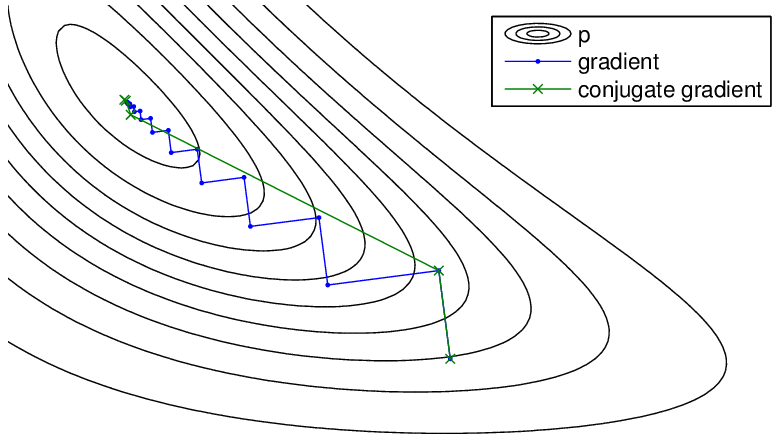
\includegraphics[width=\linewidth]{CG.png}
    
    \vspace{0.2cm}
    
    \tiny \textit{Gradient descent (blue) and conjugate gradient (green).}
\end{center}

\end{column}

\end{columns}

\end{frame}

%---------------------------------------------------------------------------------------
\begin{frame}{Key Concepts: ADMM (Alternating Direction Method of Multipliers)}

\begin{itemize}

    \item \textbf{Purpose:}  
    Solve complex optimization problems by splitting them into simpler subproblems, updated alternately.

    \vspace{0.2cm}

    \item \textbf{How it works:}  
    ADMM addresses problems of the form:  
    minimize \( f(\mathbf{x}) + g(\mathbf{z}) \)  
    subject to \( \mathbf{A}\mathbf{x} + \mathbf{B}\mathbf{z} = \mathbf{c} \).  
    It alternates updates for \(\mathbf{x}\), \(\mathbf{z}\), and the dual variable.

    \vspace{0.2cm}

    \item \textbf{Why ADMM?}  
    \begin{itemize}
        \item Handles non-smooth objectives like Total Variation (TV).
        \item Decomposes large problems into smaller, tractable steps.
        \item Efficient convergence for structured problems.
    \end{itemize}

    \vspace{0.2cm}

    \item \textbf{In this paper:}  
    ADMM solves the \textbf{Graph Total Variation (GTV)} problem for graph signal interpolation.  
    \begin{itemize}
        \item GTV preserves sharp edges by penalizing absolute differences across edges.
        \item ADMM efficiently manages the non-smooth TV regularizer.
        \item Each ADMM iteration is unrolled as a network layer, ensuring interpretability.
    \end{itemize}

\end{itemize}

\end{frame}

%---------------------------------------------------------------------------------------
\begin{frame}{Key Concepts: Datasets Used in Experiments}

\begin{columns}[c]

% Left column: Text
\begin{column}{0.7\textwidth}

\begin{itemize}

    \item \textbf{Purpose:}  
    Evaluate model performance on \textbf{demosaicking} and \textbf{image interpolation} tasks.

    \vspace{0.2cm}

    \item \textbf{Training Dataset:}  
    \textbf{DIV2K}  
    \begin{itemize}
        \item 800 high-resolution images for training, 100 for validation.
        \item Rich in detail and diversity.
        \item Patches: \(64 \times 64\), with sparse sampling (1–4\% of pixels).
    \end{itemize}

    \vspace{0.2cm}

    \item \textbf{Test Datasets:}  
    \begin{itemize}
        \item \textbf{McM} – Color demosaicking benchmark.
        \item \textbf{Kodak} – 24 high-quality natural images.
        \item \textbf{Urban100} – Urban scenes with repetitive structures.
    \end{itemize}

    \vspace{0.2cm}

    \item \textbf{In this paper:}  
    \begin{itemize}
        \item Training on DIV2K.  
        \item Testing on McM, Kodak, Urban100.  
        \item Tasks: demosaicking and interpolation.
    \end{itemize}

\end{itemize}

\end{column}

% Right column: Image
\begin{column}{0.3\textwidth}

\begin{center}
    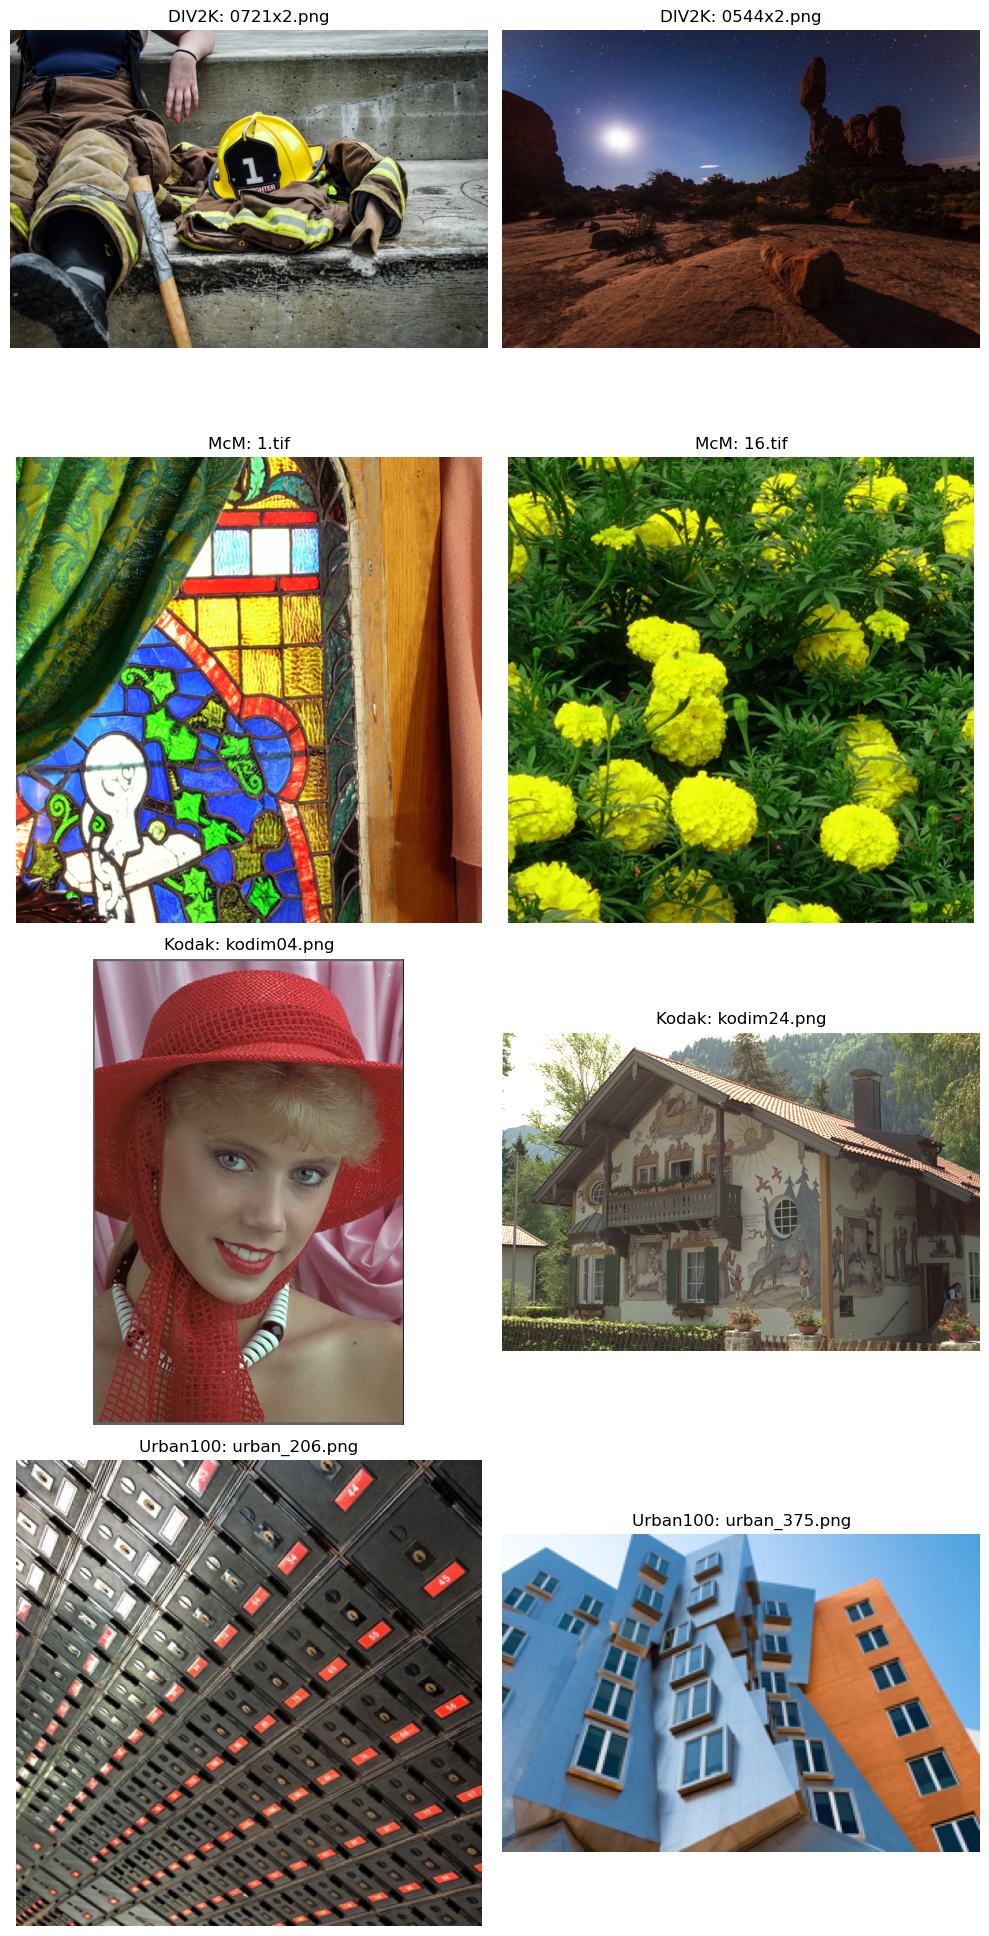
\includegraphics[width=0.7\linewidth]{dataset.png}
    
    \vspace{0.2cm}
    \tiny \textit{Sample images from DIV2K, McM, Kodak, Urban100 datasets.}
\end{center}

\end{column}

\end{columns}

\end{frame}
%---------------------------------------------------------------------------------------
\begin{frame}{Key Concepts: Task Definitions}

\begin{columns}[c]

% Left column: Image Interpolation
\begin{column}{0.5\textwidth}
\textbf{Image Interpolation}

\vspace{0.2cm}

\begin{itemize}
    \item \textbf{Purpose:} Restore missing pixels in an image from sparse or degraded inputs.
    \item \textbf{Dataset:} DIV2K, Urban100, Kodak
    \item \textbf{Challenge:} Maintain sharp edges and textures while recovering fine details.
    \item \textbf{In this paper:} Graph-based priors guide smoothness and edge preservation.
\end{itemize}

\begin{center}
    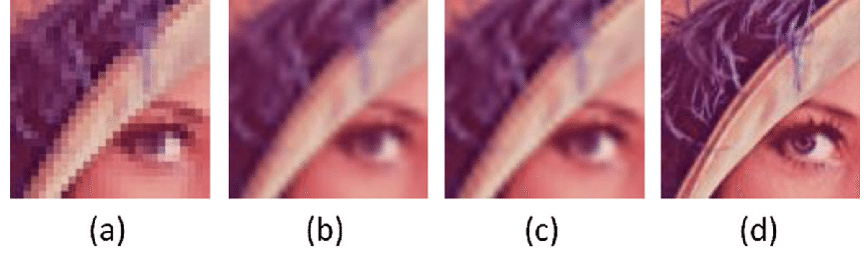
\includegraphics[width=0.9\linewidth]{Image Interpolation.png}
    
    \tiny \textit{Example of image interpolation at different levels of quality.}
\end{center}

\end{column}

% Right column: Demosaicking
\begin{column}{0.50\textwidth}
\textbf{Demosaicking}

\vspace{0.2cm}

\begin{itemize}
    \item \textbf{Purpose:} Reconstruct full RGB images from raw Bayer-patterned inputs.
    \item \textbf{Dataset:} McM, Kodak
    \item \textbf{Challenge:} Remove color artifacts and preserve fine structures.
    \item \textbf{In this paper:} Unrolled optimization ensures faithful color recovery.
\end{itemize}
\vspace{-0.2cm}
\begin{center}
    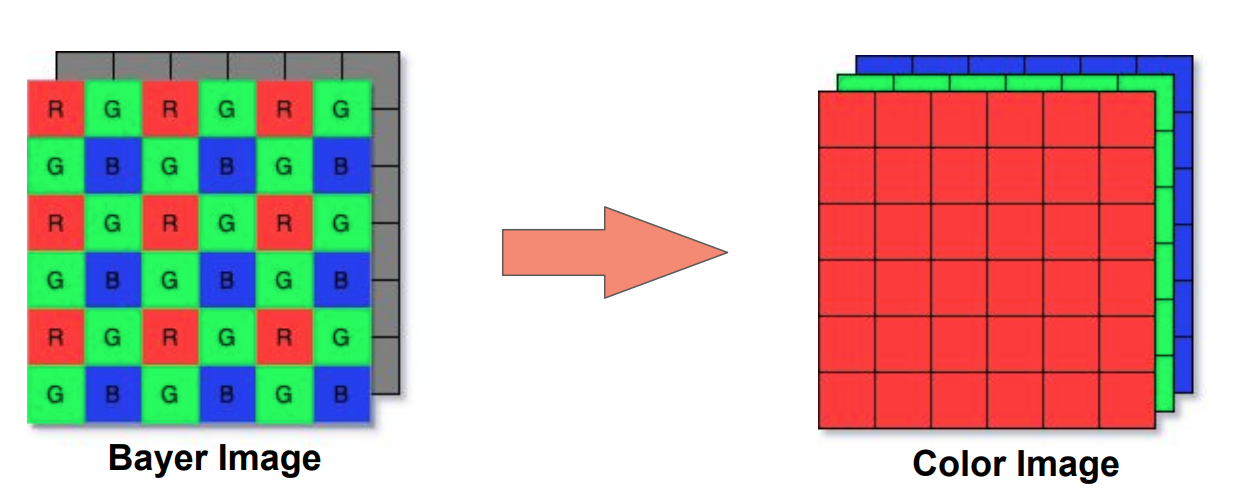
\includegraphics[width=0.7\linewidth]{Demosaicking.png}
    
    \tiny \textit{From Bayer image to reconstructed color image.}
\end{center}

\end{column}

\end{columns}

\end{frame}
%---------------------------------------------------------------------------------------
\begin{frame}{Key Concepts: Evaluation Metrics}

\begin{columns}[c]

% Left Column - PSNR
\begin{column}{0.50\textwidth}

\textbf{PSNR (Peak Signal-to-Noise Ratio)}

\begin{itemize}
    \item Measures pixel-level fidelity between the reconstructed and reference images.
    
    \item Formula:
    \vspace{-0.2cm}
    {\scriptsize
    \[
    PSNR = 10 \log_{10} \left( \frac{MAX_I^2}{MSE} \right)
    \]
    }
    \vspace{-0.6cm}
    \item $MAX_I$: maximum pixel value (e.g., 255)  
    \item Higher PSNR $\rightarrow$ Less distortion  
    \item Common in image compression and reconstruction
    \item \textbf{Not reflecting human perception}
    \item Insensitive to structural or perceptual distortions
\end{itemize}

\end{column}

% Right Column - SSIM
\begin{column}{0.50\textwidth}

\textbf{SSIM (Structural Similarity Index)}

\begin{itemize}
    \item Evaluates perceptual similarity: Luminance, Contrast \& Structure
    
    \item Formula (simplified):
    \vspace{-0.2cm}
    {\scriptsize
    \[
    SSIM(x, y) = \frac{(2\mu_x\mu_y + C_1)(2\sigma_{xy} + C_2)}{(\mu_x^2 + \mu_y^2 + C_1)(\sigma_x^2 + \sigma_y^2 + C_2)}
    \]
    }
    \vspace{-0.6cm}
    \item Values in $[0, 1]$  
    \item Closer to $1$ $\rightarrow$ More similarity
\end{itemize}

\begin{center}
    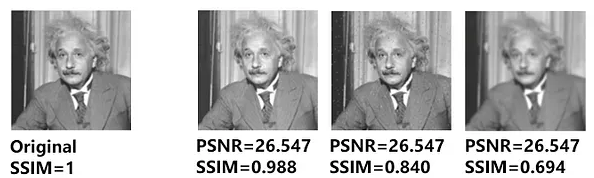
\includegraphics[width=0.7\linewidth]{PSNRvsSSIM.png}
\end{center}
\vspace{-0.2cm}
\tiny \textit{Images with the same PSNR but decreasing SSIM values show visible perceptual degradation.}

\end{column}

\end{columns}

\end{frame}

%---------------------------------------------------------------------------------------
\begin{frame}{Related Work: Feedback-based Graph Learning}

\begin{columns}[c]

% Left Column - Main Idea
\begin{column}{0.48\textwidth}

\textbf{Inpainting-Driven Graph Learning via Explainable Neural Networks}  
\\\textit{Lingxiao Zhang, Gene Cheung, Xavier Bresson, and Ching-Yun Ko - 2025}

\vspace{0.5cm}
\textbf{Main contributions:}
\begin{itemize}
    \item Learns both signal and graph \textbf{jointly}, without ground-truth.
    \item Designed for \textbf{temporal signals} (e.g., fMRI, sensors).
    \item \textbf{Feedback loop:} signal recovery $\rightarrow$ graph update $\rightarrow$ repeat.
    \item Fully \textbf{unsupervised}, interpretable and task-adaptive.
\end{itemize}

\end{column}

% Right Column - Comparison + Visual
\begin{column}{0.52\textwidth}

\textbf{Compared to our main paper:}
\begin{itemize}
    \item Focus on \textbf{dynamic graphs} vs static.
    \item \textbf{Closed-loop unrolling} vs fixed iteration blocks.
    \item \textbf{Unsupervised} learning vs supervised training with ground-truth signals.
    \item Full \textbf{end-to-end feedback architecture} vs modular design (graph then signal).
\end{itemize}

\vspace{-0.2cm}
\begin{center}
    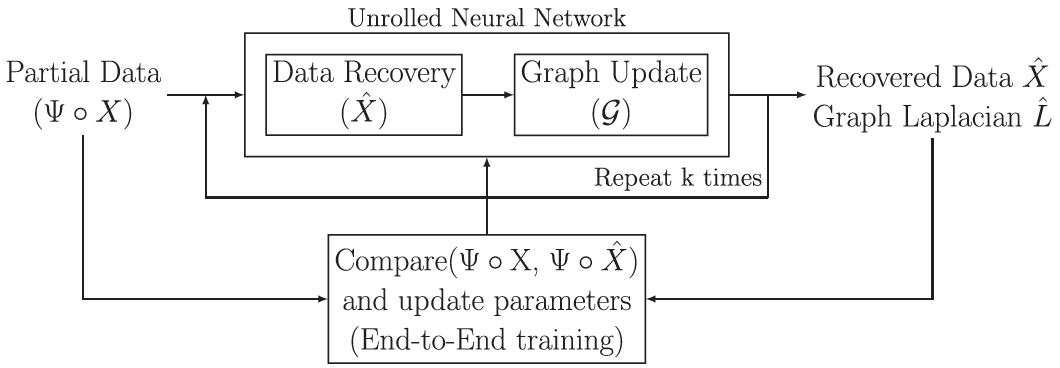
\includegraphics[width=0.85\linewidth]{paper2.png}
\\\tiny \textit{Joint unrolling of signal recovery and graph learning.}
\end{center}


\end{column}

\end{columns}

\end{frame}
\end{document}